\documentclass[tikz,border=10pt]{standalone}
\usepackage{amsmath}
\usetikzlibrary{positioning, fit}

\begin{document}

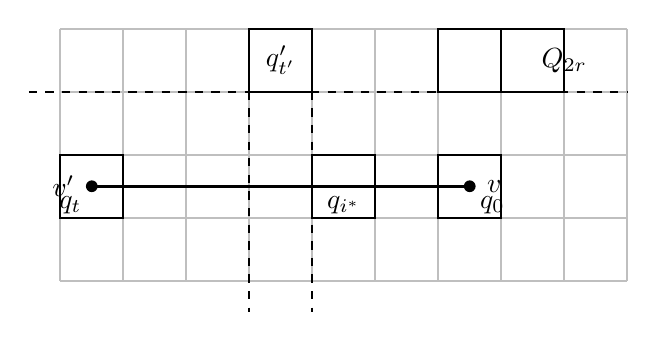
\begin{tikzpicture}[scale=0.8, thick]

% Define grid lines
\draw[gray!50] (0,0) grid (9,4);

% Draw highlighted cells
\filldraw[fill=white, draw=black] (3,3) rectangle (4,4); % q'_{t'}
\filldraw[fill=white, draw=black] (6,1) rectangle (7,2); % v
\filldraw[fill=white, draw=black] (0,1) rectangle (1,2); % v'
\filldraw[fill=white, draw=black] (4,1) rectangle (5,2); % q_{i^*}
\filldraw[fill=white, draw=black] (6,3) rectangle (7,4); % part of Q_{2r}
\filldraw[fill=white, draw=black] (7,3) rectangle (8,4); % part of Q_{2r}

% Draw diagonal line from v' to v
\draw[very thick] (0.5,1.5) -- (6.5,1.5) -- (6.5,1.5);
\draw[very thick] (0.5,1.5) -- (6.5,1.5) -- (6.5,1.5);

% Label points
\node[circle, fill=black, inner sep=1.5pt, label={left:$v'$}] at (0.5,1.5) {};
\node[circle, fill=black, inner sep=1.5pt, label={right:$v$}] at (6.5,1.5) {};

% Labels for specific nodes
\node at (3.5,3.5) {$q'_{t'}$};
\node at (0.5,1.5) [below left] {$q_t$};
\node at (4.5,1.5) [below] {$q_{i^*}$};
\node at (6.5,1.5) [below right] {$q_0$};

% Label for Q_{2r}
\node at (8,3.5) {$Q_{2r}$};

% Draw vertical and horizontal lines through q'_{t'}
\draw[dashed] (3,3) -- (3,-0.5);
\draw[dashed] (4,3) -- (4,-0.5);
\draw[dashed] (-0.5,3) -- (9,3);

\end{tikzpicture}

\end{document}